\subsection{One dimensional hydrogen chain}
We now move to one of the simplest extended \emph{ab-initio} systems, a hydrogen chain in one dimension with periodic boundary conditions. 
%%HHZ: We don't need to say exact eigenstates stuff.
%In the absence of availability of exact eigenstates, the example will highlight the effectiveness of the N-AIDMD approach. 
We consider the case of $10$ atoms and work in a regime where the inter-atomic distance $r$ is 
relatively large ($r=1.5$ to $3.0$ \AA), such that the system is potentially well described by a 1-band Hubbard model 
in terms of primarily $s$-like orbitals, whose form we discuss here. 

\HHZ{General comment for all of us: This is a physics paper, and the readers will mostly be physicists. Therefore, I think emphasizing physics quantities is more important than machine learning terminologies. I would say PHYSICS TERM (MACHINE LEARNING TERM) instead of MACHINE LEARNING TERM (PHYSICS TERM).} 
\lucas{What are you talking about specifically?}  \HHZ{I meant the following paragraph.}

For a given $r$, we first obtain single-particle Kohn-Sham orbitals from a set of spin-unrestricted and 
spin-restricted DFT-PBE calculations. The localized orbital basis upon which the density matrices (descriptors) 
are evaluated is obtained by generating intrinsic atomic orbitals (IAO) from the Kohn-Sham orbitals 
orthogonalized using the L\"owdin procedure. The resulting orbitals are shown in Fig.~\ref{fig:h10orb}. These are the orbitals that enter the 1-band Hubbard Hamiltonian. 

%\begin{figure}[]
%\centering
%\subfigure[KS 1]{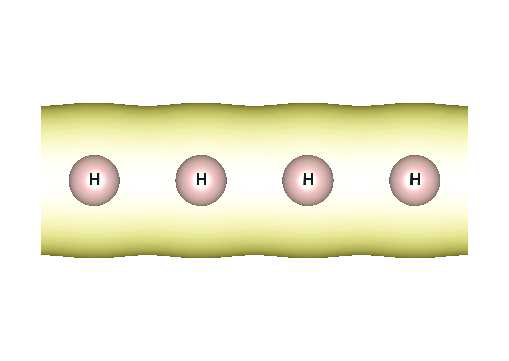
\includegraphics[width=0.20\linewidth]{./Figures/h4_ks1.png}}\quad
%\subfigure[KS 2]{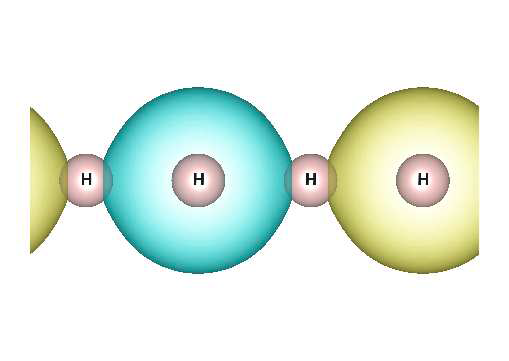
\includegraphics[width=0.20\linewidth]{./Figures/h4_ks2.png}}\quad
%\subfigure[KS 3]{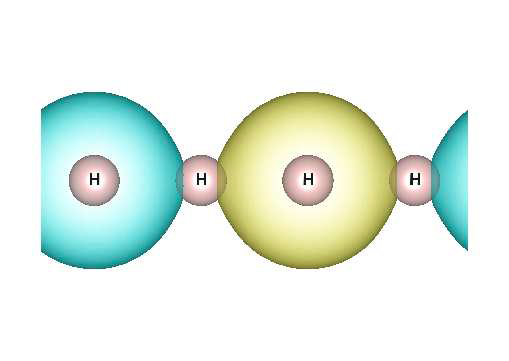
\includegraphics[width=0.20\linewidth]{./Figures/h4_ks3.png}}\quad
%\subfigure[KS 4]{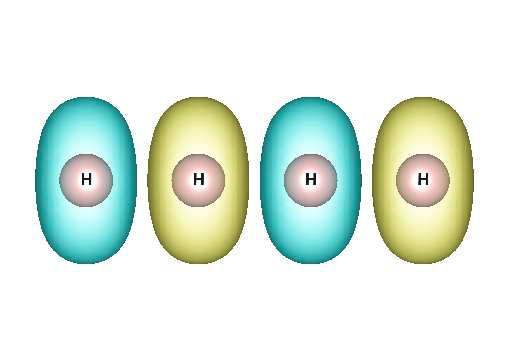
\includegraphics[width=0.20\linewidth]{./Figures/h4_ks4.png}}
%\\
%\subfigure[Wannier 1]{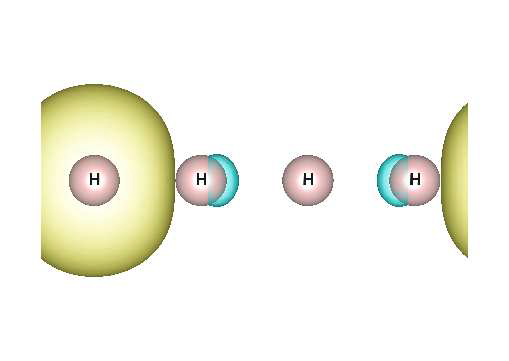
\includegraphics[width=0.20\linewidth]{./Figures/h4_wan1.png}}\quad
%\subfigure[Wannier 2]{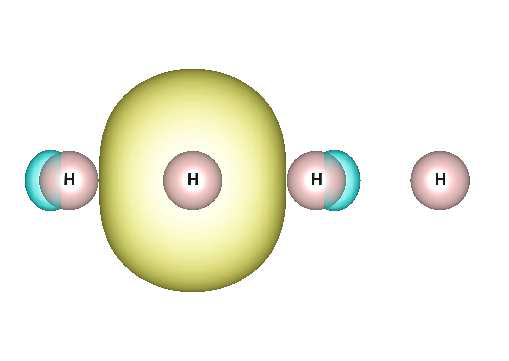
\includegraphics[width=0.20\linewidth]{./Figures/h4_wan2.png}}\quad
%\subfigure[Wannier 3]{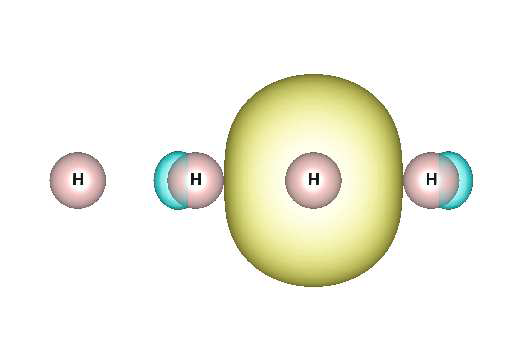
\includegraphics[width=0.20\linewidth]{./Figures/h4_wan3.png}}\quad
%\subfigure[Wannier 4]{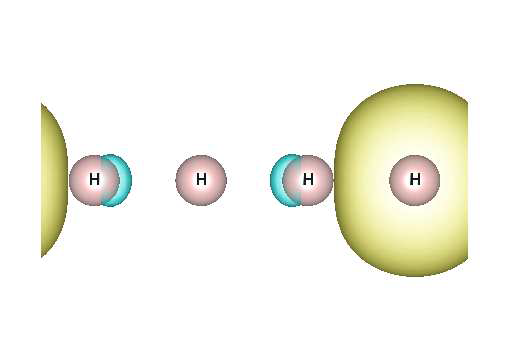
\includegraphics[width=0.20\linewidth]{./Figures/h4_wan4.png}}
%\caption{\HJC{Put IAO here} Kohn-Sham orbitals (upper panel) from DFT calculations with PBE exchange-exchange correlation functional, and Wannier orbitals (lower panel) constructed through a unitary transformation of Kohn-Sham orbitals.}\label{fig:h4orb}
%\end{figure}

\begin{figure}[]
\centering
\subfigure[Separation = $1$ \AA]{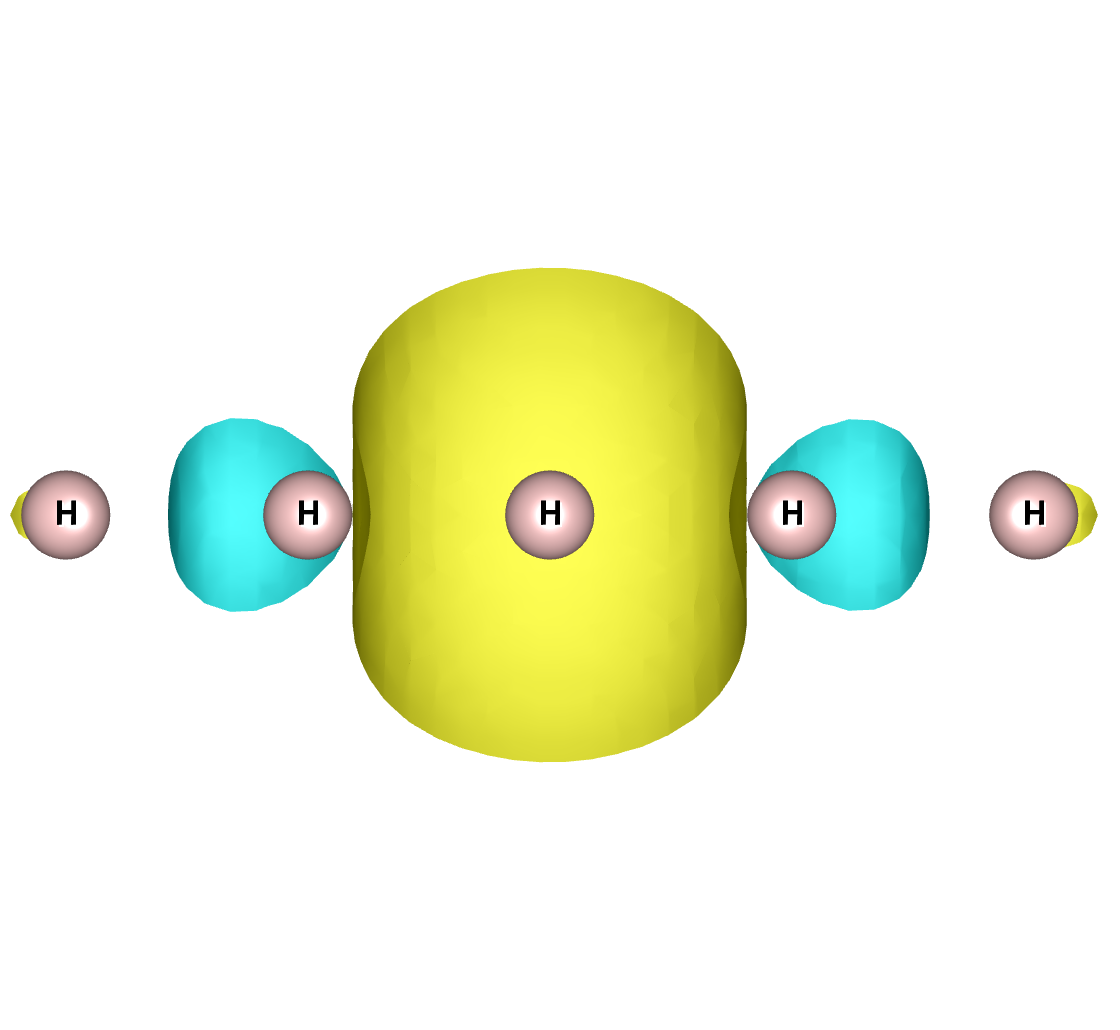
\includegraphics[width=0.28\linewidth]{{./Figures/length1_h_paper_view.orb5}.png}}\quad
\subfigure[Separation = $1.5$ \AA]{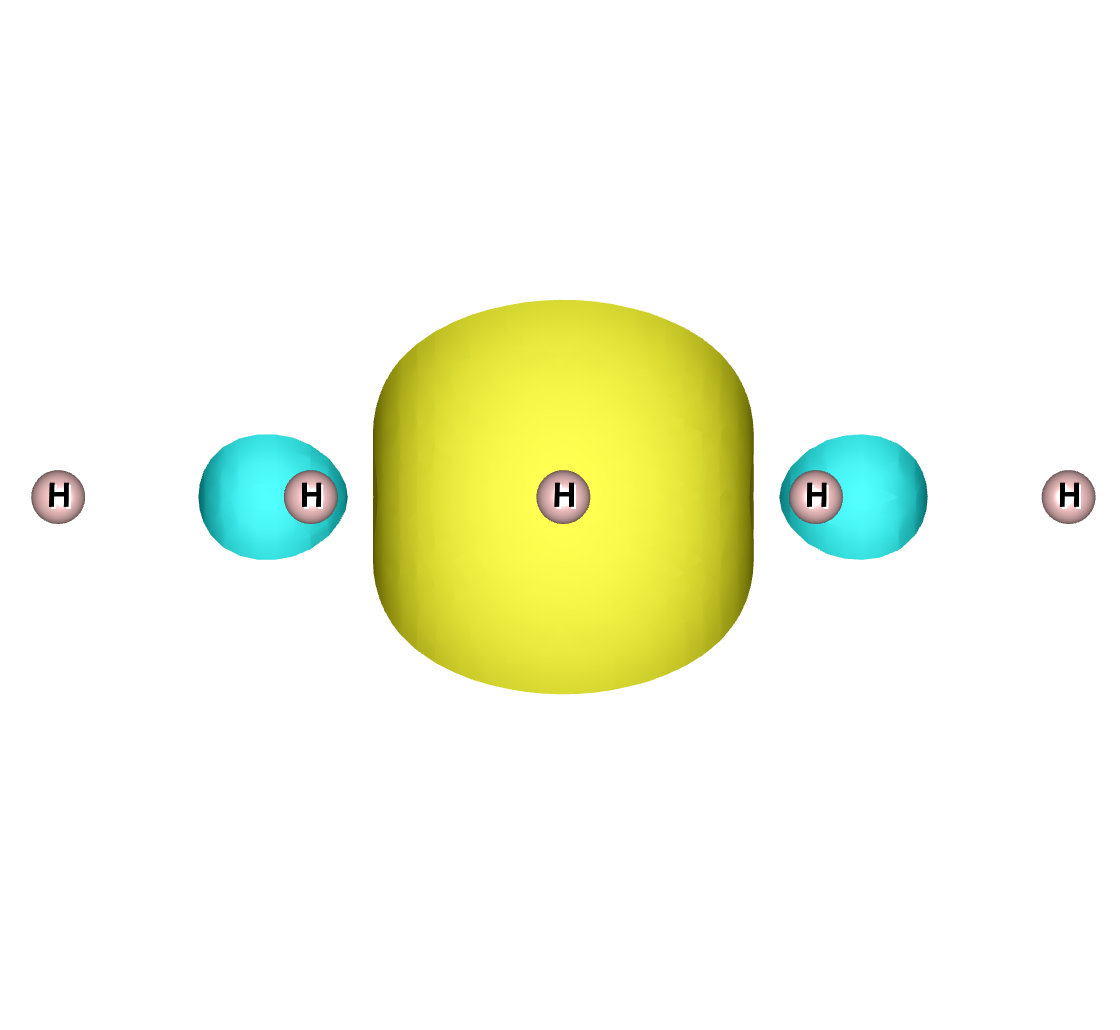
\includegraphics[width=0.28\linewidth]{{./Figures/length1.5_h_paper_view.orb5}.png}}\quad
\subfigure[Separation = $2$ \AA]{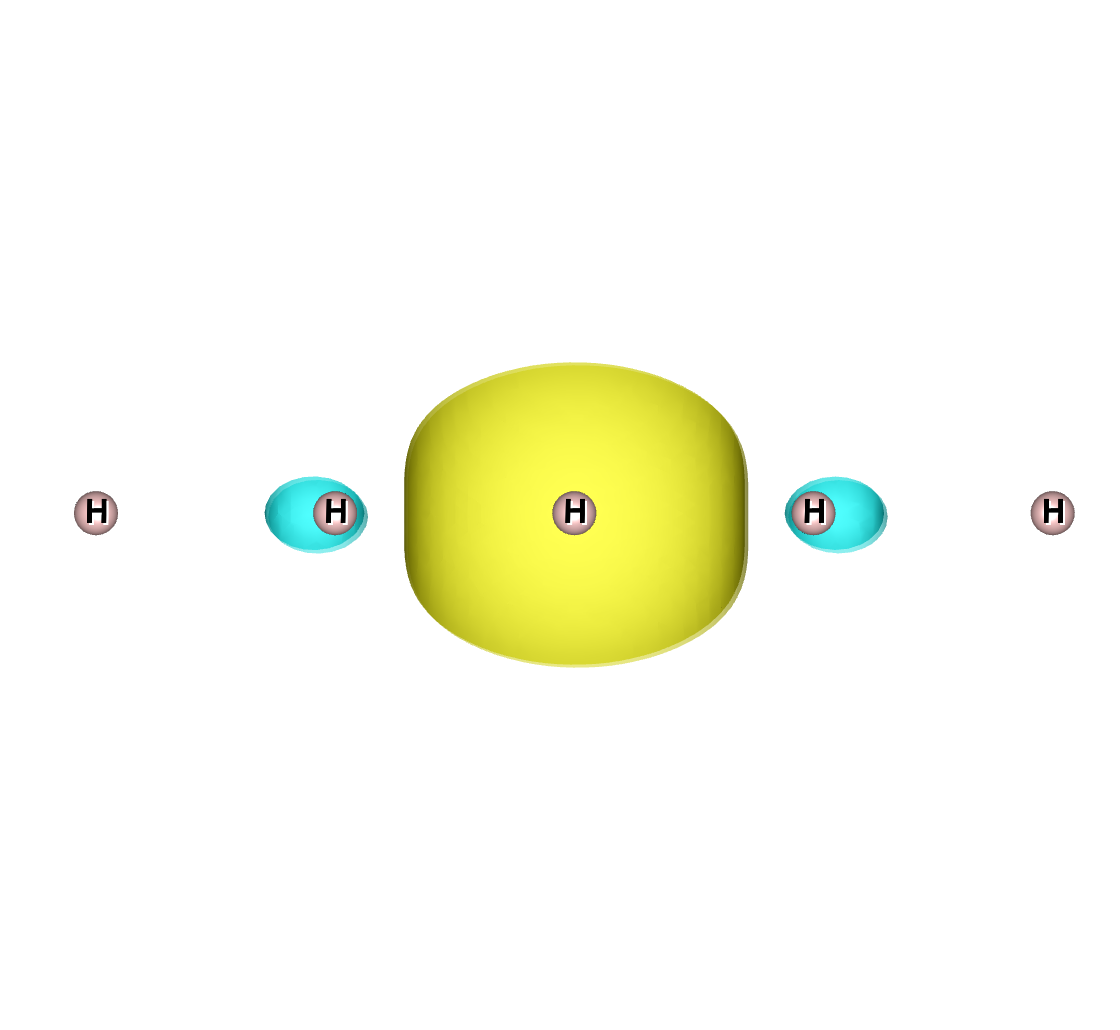
\includegraphics[width=0.28\linewidth]{{./Figures/length2_h_paper_view.orb5}.png}}
\caption{\HJC{Put IAO here Done -Kiel} Orthogonalized intrinsic atomic orbitals for interatomic hydrogen separation distances equal to $1$, $1.5$, and $2$ \AA \:respectively}\label{fig:h10orb}
\end{figure}

To generate a database of wavefunctions needed for the N-AIDMD, we produce a set of Slater-Jastrow 
wavefunctions consisting of singles- and doubles- excitations to the Slater determinant, 
\begin{subequations}
\begin{eqnarray}
| s \rangle = & \Big[a^\dagger_{i \sigma} a_{k \sigma}   | KS \rangle \Big]e^J \,,\\
| d \rangle = & \: \Big[a^\dagger_{i \sigma} a^\dagger_{j \sigma'} a_{k \sigma'} c_{l \sigma}   | KS \rangle\Big]e^J ,
\end{eqnarray}
\end{subequations}
where $|KS\rangle$ is the Stater determinant of occupied Kohn-Sham orbitals, $\sigma$ and $\sigma'$ are spin indices, 
$a_{i}^\dagger$ ($a_{i}$) is a single-electron creation (destruction) corresponding to Kohn-Sham orbitals, 
and $e^J$ is the Jastrow factor which was optimized using variational Monte Carlo. 
We compute the energies (expectation values of the Hamiltonian) and the reduced density matrices (descriptors) on all the wave functions. 
%Then, having computed the energies (expectation values of the Hamiltonian) and corresponding 
%descriptors for these wavefunctions we verify the independence of the $U$ and $t$ descriptors. 
We then fit the 1-band Hubbard Hamiltonian using least-squares fitting according to the N-AIDMD formalism described in Sec. 2. %, as part of the formalism described in sec. 2. 

\begin{figure}
\centering
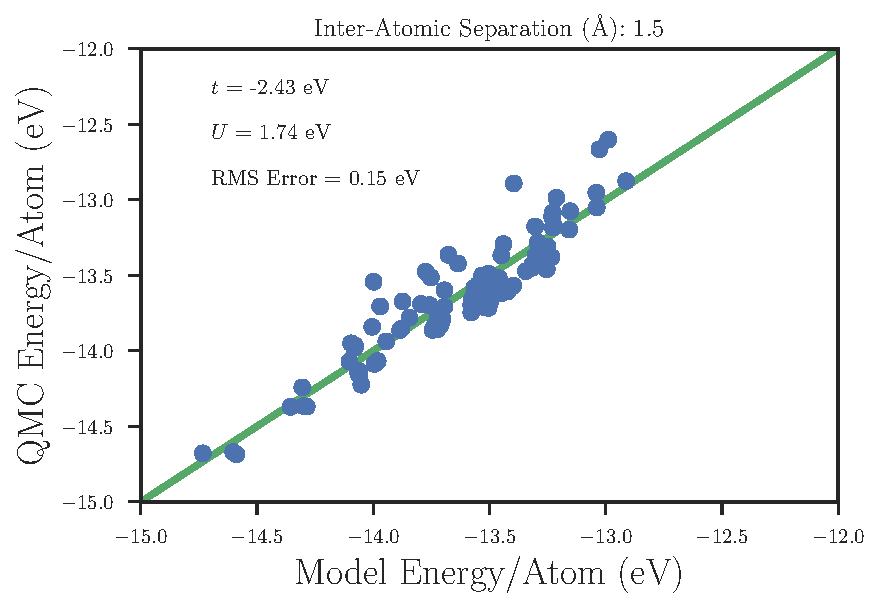
\includegraphics[scale=0.5]{{./Figures/H_chain_fit_model_length1.5_tUs}.pdf}
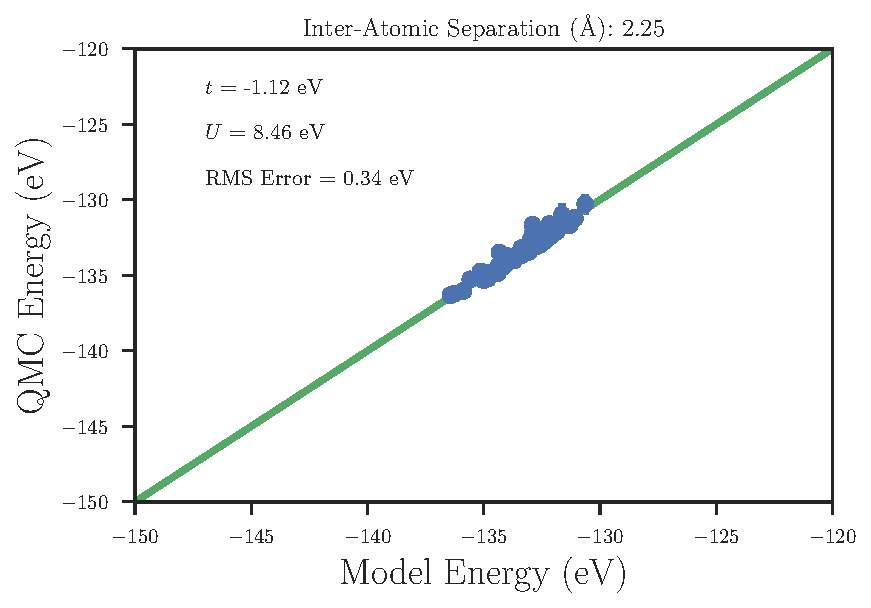
\includegraphics[scale=0.5]{{./Figures/H_chain_fit_model_length2.25_tUs}.pdf}
\caption{\HJC{Put model vs ab-initio plots here. Done -Kiel} DMC energy vs. model energy for the H$_{10}$ chain at 1.5 \AA \:(left) and 2.25 \AA \:(right). Note that the energy range narrows significantly for larger interatomic separation. \HHZ{Could you change to total energy instead of energy per atom?}}\label{fig:fit_quality}
\end{figure}

Fig.~\ref{fig:fit_quality} shows our N-AIDMD fits for two representative $r$. As expected, the RMS error 
is significantly smaller for larger $r$, verifying the effectiveness of the Hubbard model 
in this limit. 
Fig.~\ref{fig:Parameters-vs-Bond-t} also shows trends of the fitted value of $t$ 
and $U$ as a function of $r$. 
Consistent with physical intuition, $t$ decreases towards zero at larger $r$
and the value of $U/t$ rises. 

The single band Hubbard model does not describe hydrogen chain well at small distance. 
The one dimensional Hubbard model with $U/|t|>0$ will always result in an Mott insulating state. 
However, the metal-to-insulator transition happens at $r_c=\sim1.8$\AA~ for a hydrogen chain \cite{Stella2011}. 
This indicates that at small distance, higher energy orbitals (e.g. P, D, etc) play nontrivial role in stabilizing the metallic state of hydrogen, instead of merely renormalizing the effective strength of U. 
Meanwhile, at small distance, other interaction terms like nearest neighbor Coulomb interaction and Heisenberg exchange interaction also become important at $r<r_c$ \cite{ZhengThesis}. 

\begin{figure}
\centering
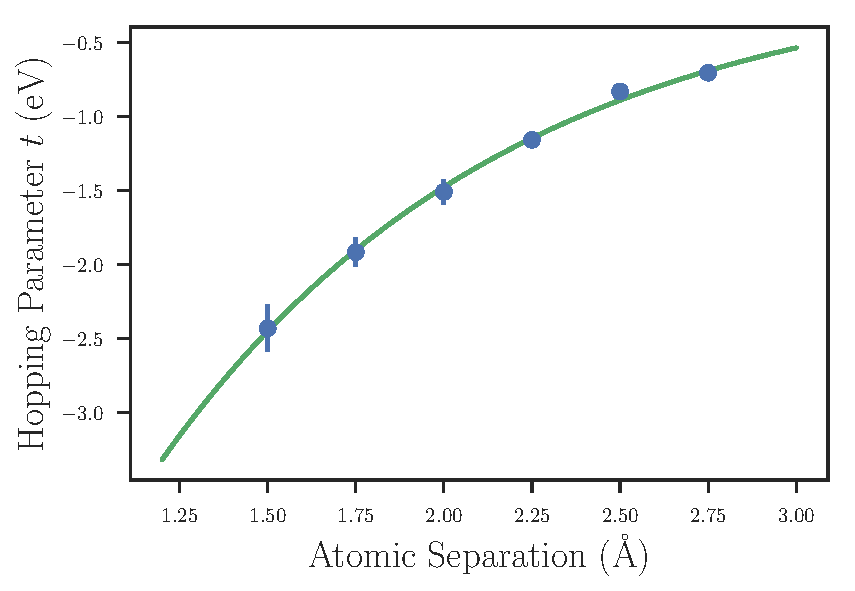
\includegraphics[scale=0.5]{./Figures/fitted_t_values_no_annotate_h10_chain.pdf}
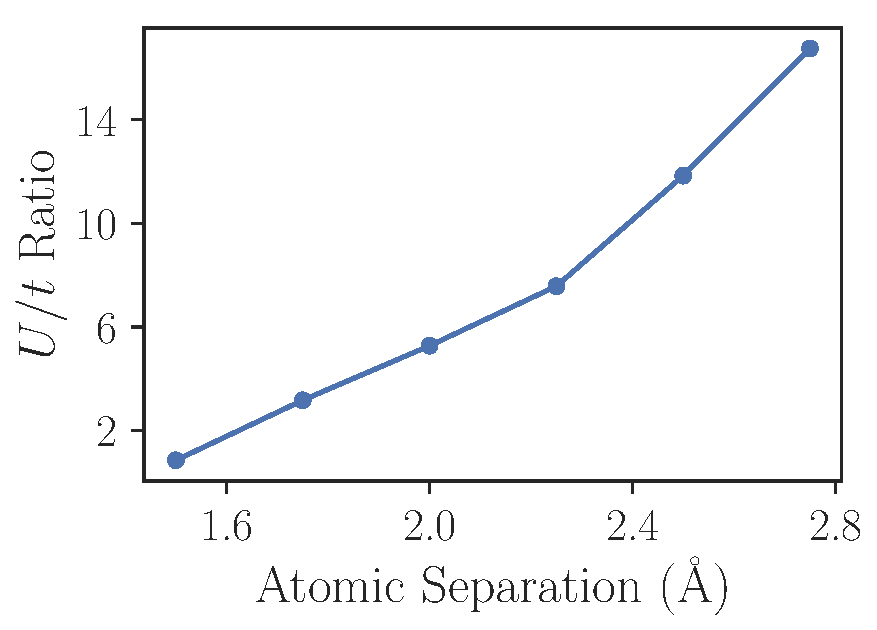
\includegraphics[scale=0.5]{./Figures/Ust_ratio_vs_separation_h_chain.pdf}
\caption{\HJC{Put t vs r and U/t vs r Done -Kiel} (Left) The one-body hopping $t$ parameter as a function of interatomic distance for the periodic H$_{10}$ chain, obtained from a fitted $U$-$t$ model. $t$ declines to zero as $r$ increases. (Right) The ratio $U/t$ for the fitted parameter values as a function of interatomic separation. The ratio is small at lower bond-lengths, where $t$ is more relevant in describing the system, and larger at longer bond-lengths, where inter-site hopping is less significant. }\label{fig:Parameters-vs-Bond-t}
\end{figure}
